%!TEX root=masterproef.tex

\chapter{hello.foo}
\label{appendix:hello-srcs}

Deze bijlage bevat de belangrijkste gegenereerde code van \ttt{hello.foo},
ge\"introduceerd in hoofdstuk \ref{chapter:implementatie}, alsook een
visualisatie van het het uitgewerkte \ttt{nodes}-domein in het SM.

\section{main.c}
\vspace{-5mm}
\begin{listing}[H]
  \begin{minted}[linenos,frame=lines,framesep=2mm,fontsize=\footnotesize]{c}
#include "main.h"
//  init and application_step
void init(void) {
  // add framework init here
  nodes_init();
  mesh_on_receive(payload_parser_parse);
}
void application_step(void) {
  // add application specific code here
}
/*
  starting point
  please don't change anything beyond this point.
*/
int main(void) {
  init();
  nodes_scheduler_init();
  while(TRUE) {
    // your application gets its share
    application_step();
    // nodes logic execution hook
    nodes_process();
    xbee_receive();
  }
  return 1;
}
void nodes_scheduler_init(void) {
  nodes_schedule_all(interval, step);
}
  \end{minted}
  \vspace{-5mm}
  \caption{Generatie van \ttt{hello.foo}: main.c}
\end{listing}

\section{constants.h}
\vspace{-5mm}
\begin{listing}[H]
  \begin{minted}[linenos,frame=lines,framesep=2mm,fontsize=\footnotesize]{c}
#ifndef __CONSTANTS_H
#define __CONSTANTS_H

#define interval 1000

#endif
  \end{minted}
  \vspace{-5mm}
  \caption{Generatie van \ttt{hello.foo}: constants.h}
\end{listing}

\section{node\_t.h}
\vspace{-5mm}
\begin{listing}[H]
  \begin{minted}[linenos,frame=lines,framesep=2mm,fontsize=\footnotesize]{c}
#ifndef __NODE_T_H
#define __NODE_T_H

#include "moose/bool.h"
// THE node type
typedef struct node_t {
  // domain properties
  uint8_t id;
  uint16_t address;
  // extended properties for hello
  uint8_t sequence;
} node_t;
void init_node(node_t* node);

#endif
  \end{minted}
  \vspace{-5mm}
  \caption{Generatie van \ttt{hello.foo}: node\_t.h}
\end{listing}

\section{node\_t.c}
\vspace{-5mm}
\begin{listing}[H]
  \begin{minted}[linenos,frame=lines,framesep=2mm,fontsize=\footnotesize]{c}
#include "node_t.h"
void init_node(node_t* node) {
  node->sequence = 0;
}
  \end{minted}
  \vspace{-5mm}
  \caption{Generatie van \ttt{hello.foo}: node\_t.c}
\end{listing}

\section{nodes-hello.h}
\vspace{-5mm}
\begin{listing}[H]
  \begin{minted}[linenos,frame=lines,framesep=2mm,fontsize=\footnotesize]{c}
#ifndef __NODES_HELLO_H
#define __NODES_HELLO_H

#include "nodes.h"
#include "includes.h"
void step(node_t* node);

#endif
  \end{minted}
  \vspace{-5mm}
  \caption{Generatie van \ttt{hello.foo}: nodes-hello.h}
\end{listing}

\section{nodes-hello.c}
\vspace{-5mm}
\begin{listing}[H]
  \begin{minted}[linenos,frame=lines,framesep=2mm,fontsize=\footnotesize]{c}
#include "nodes-hello.h"
void step(node_t* node) {
  if((node->sequence < 10)) {
    node->sequence++;
  }
}
  \end{minted}
  \vspace{-5mm}
  \caption{Generatie van \ttt{hello.foo}: nodes-hello.c}
\end{listing}

\section{Het \ttt{nodes}-domein in het SM}
\label{section:nodes.sm}

Figuur \ref{fig:nodes.sm} toont de volledige inhoud van het \ttt{nodes}-domein,
zoals dit gedefinieerd is in het geval van \ttt{hello.foo}. De uitbreiding van
de definitie van een knoop met de \ttt{sequence}-eigenschap is uitvergroot
weergegeven.

\begin{figure}[H]
  \centering
  \begin{overpic}[width=0.74\linewidth]{resources/nodes_sm.pdf}
    \put(140,350){
\setlength{\fboxsep}{0pt}%
\setlength{\fboxrule}{1pt}%
\fbox{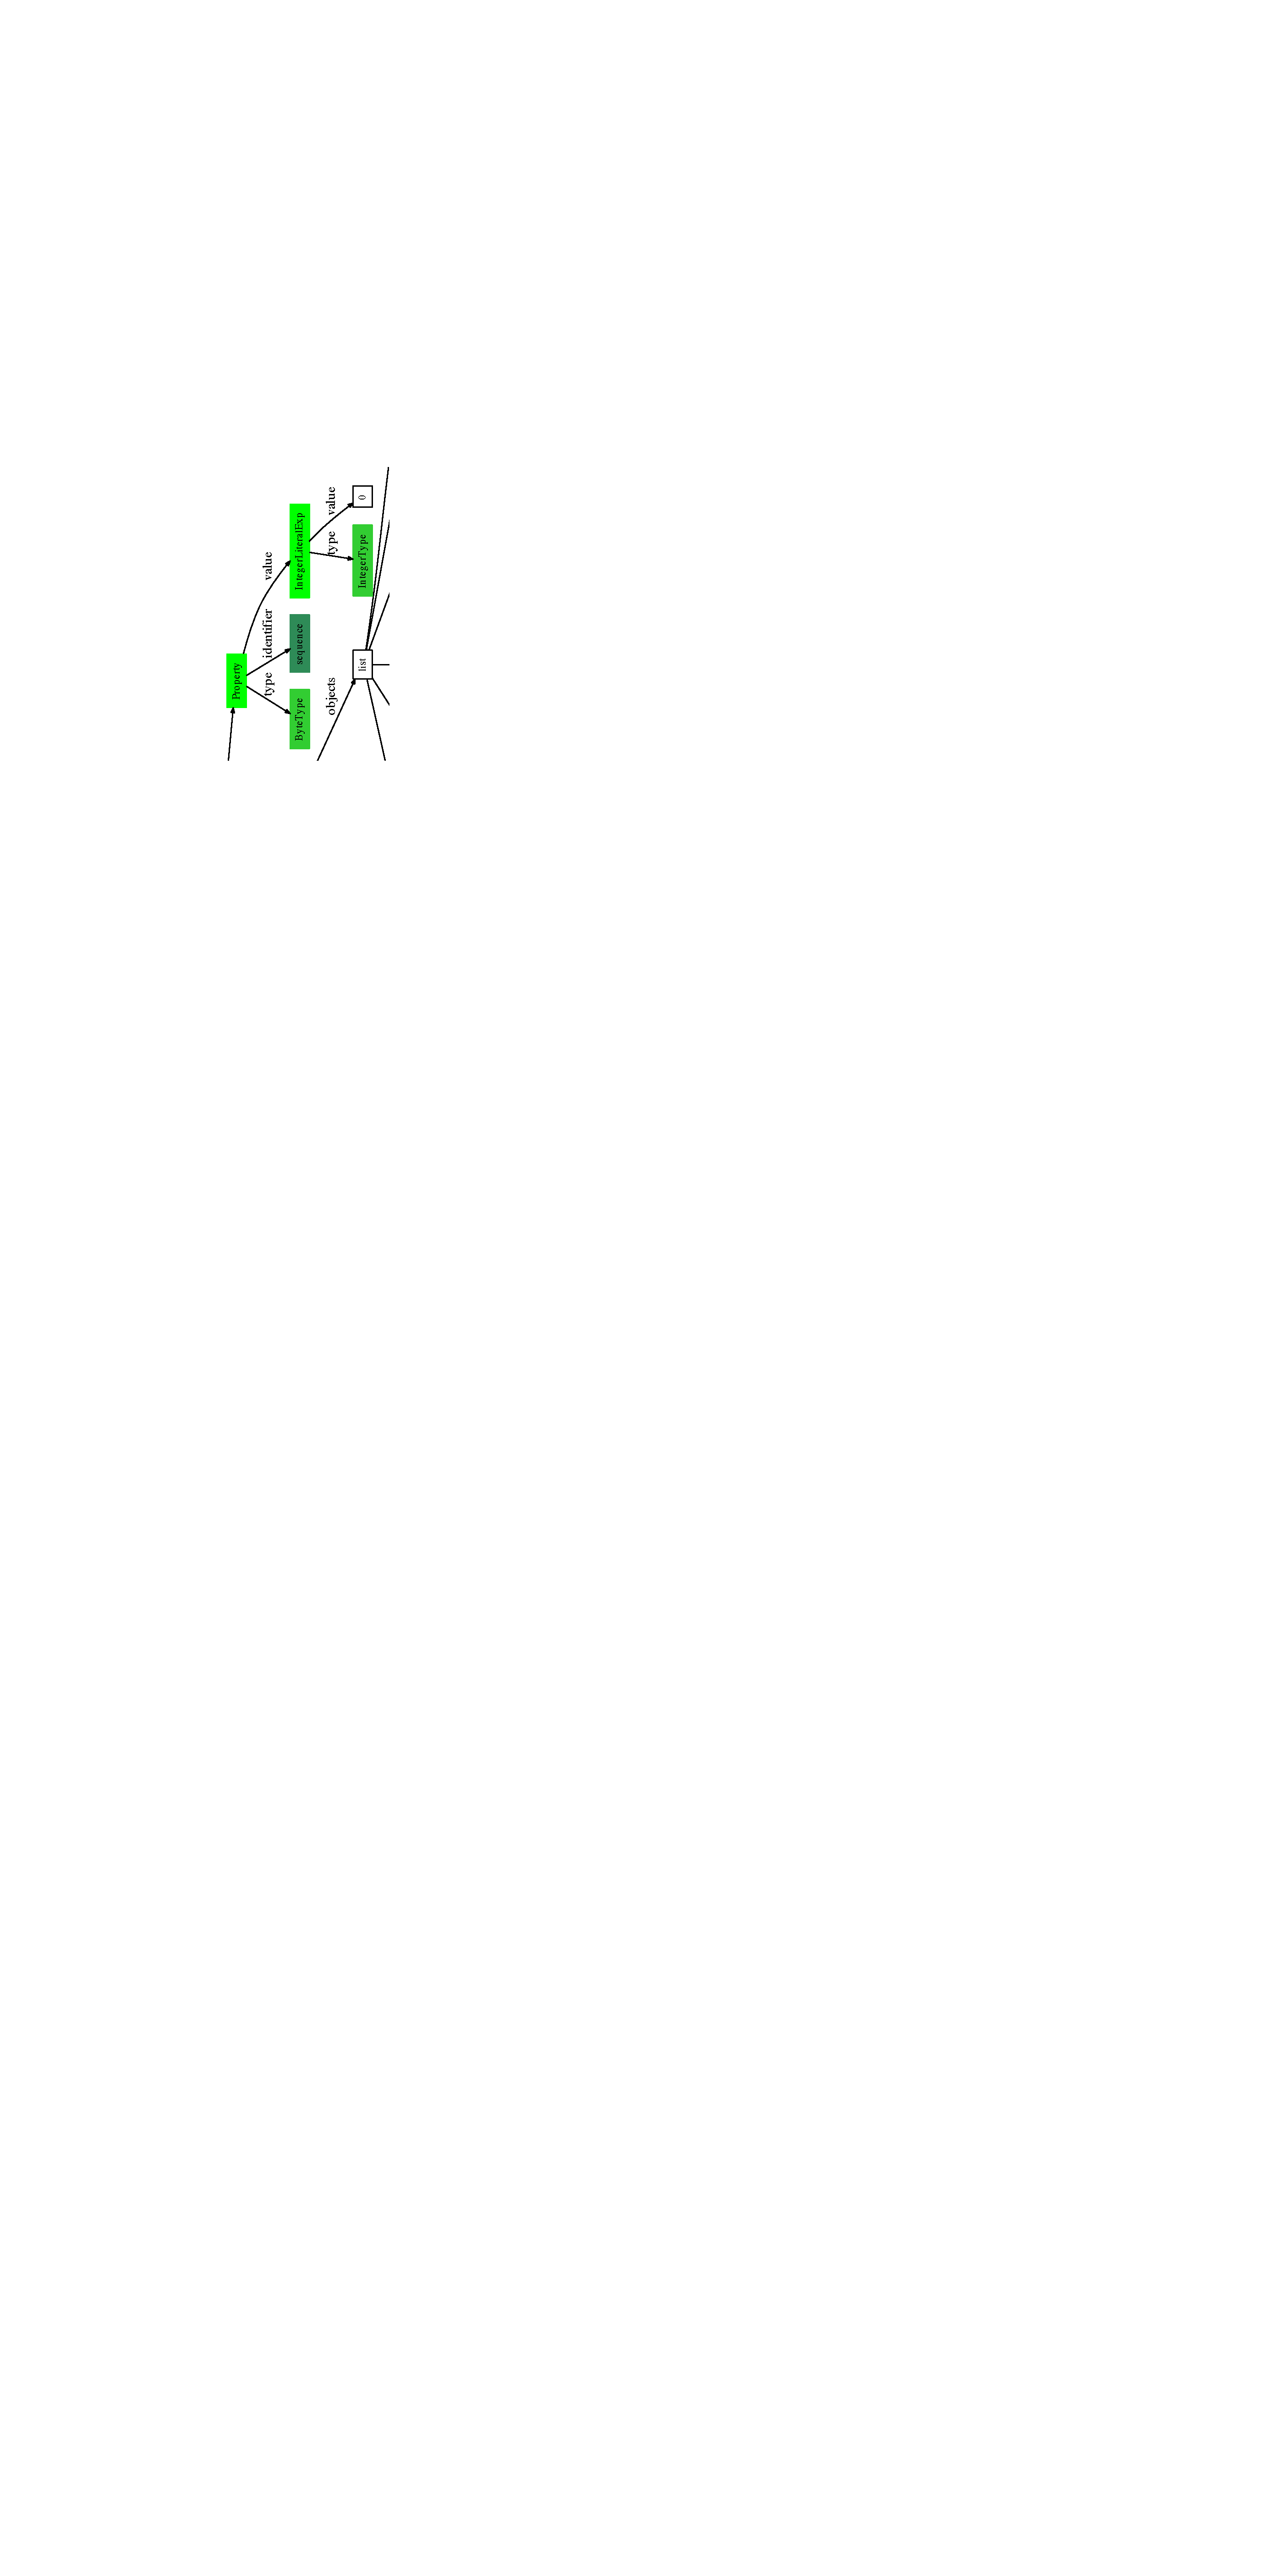
\includegraphics[scale=0.75]{resources/nodes_sm_detail.pdf}}%
    }  
  \end{overpic}
  \caption{Het \ttt{nodes}-domein in het SM voor \ttt{hello.foo} }
  \label{fig:nodes.sm}
\end{figure}
